\documentclass[12pt,a4paper]{article}

% ─── Page Layout ───────────────────────────────────────────────────────────────
\usepackage[a4paper, margin=0.8in, headheight=14pt]{geometry}

% ─── Fonts (XeLaTeX) ───────────────────────────────────────────────────────────
\usepackage{fontspec}
\usepackage{unicode-math}
\setmainfont{TeX Gyre Pagella}
\setmonofont[Scale=0.88]{TeX Gyre Cursor}
\setmathfont{Latin Modern Math}

% ─── Packages ──────────────────────────────────────────────────────────────────
\usepackage{xcolor}
\usepackage{colortbl}
\usepackage{titlesec}
\usepackage{enumitem}
\usepackage{tabularx}
\usepackage{booktabs}
\usepackage{array}
\usepackage{amsmath}
\usepackage{tikz}
\usetikzlibrary{shapes.geometric, arrows.meta, positioning, calc, fit}
\usepackage{tcolorbox}
\tcbuselibrary{skins, breakable}
\usepackage{hyperref}
\usepackage{fancyhdr}
\usepackage{graphicx}
\usepackage{microtype}
\hyphenpenalty=10000
\exhyphenpenalty=10000
\sloppy
\usepackage{caption}
\usepackage{setspace}
\usepackage{multirow}
\usepackage{tocloft}

% ─── Q&A helper ────────────────────────────────────────────────────────────────
\newcommand{\Q}[1]{\textbf{#1}\par\noindent\ignorespaces}

% ─── Colour Palette ────────────────────────────────────────────────────────────
\definecolor{myred}{RGB}{196,30,58}
\definecolor{mydark}{RGB}{30,30,50}
\definecolor{mygreen}{RGB}{14,120,80}
\definecolor{myteal}{RGB}{0,130,140}
\definecolor{myamber}{RGB}{180,100,0}
\definecolor{mypurple}{RGB}{100,30,160}
\definecolor{mygray}{RGB}{246,247,249}
\definecolor{mgframe}{RGB}{180,185,200}
\definecolor{watermark}{RGB}{145,150,170}
\definecolor{hdrred}{RGB}{250,232,235}
\definecolor{hdrgreen}{RGB}{220,244,233}
\definecolor{hdrteal}{RGB}{220,242,244}
\definecolor{hdramber}{RGB}{253,242,215}
\definecolor{hdrpurple}{RGB}{238,228,255}
\definecolor{hdrgray}{RGB}{238,240,245}
\definecolor{rowalt}{RGB}{250,251,253}

% ─── Section Formatting ────────────────────────────────────────────────────────
\titleformat{\section}
  {\large\bfseries\color{myred}}{\thesection.}{0.5em}{}
  [\vspace{1pt}{\color{myred}\rule{\linewidth}{0.8pt}}]
\titleformat{\subsection}
  {\normalsize\bfseries\color{myteal}}{\thesubsection}{0.5em}{}
\titlespacing*{\section}{0pt}{18pt}{7pt}
\titlespacing*{\subsection}{0pt}{11pt}{4pt}
\setlength{\parindent}{0pt}
\setlength{\parskip}{4pt}

% ─── TOC Styling ───────────────────────────────────────────────────────────────
\renewcommand{\cfttoctitlefont}{\large\bfseries\color{myred}}
\renewcommand{\cftaftertoctitle}{\par\noindent{\color{myred}\rule{\linewidth}{0.8pt}}}
\setlength{\cftbeforetoctitleskip}{0pt}
\setlength{\cftaftertoctitleskip}{6pt}
\renewcommand{\cftsecfont}{\normalsize\bfseries\color{mydark}}
\renewcommand{\cftsecpagefont}{\normalsize\bfseries\color{mydark}}
\renewcommand{\cftsecleader}{\cftdotfill{\cftdotsep}}
\setlength{\cftbeforesecskip}{7pt}
\renewcommand{\cftsubsecfont}{\small\color{mydark}}
\renewcommand{\cftsubsecpagefont}{\small\color{mydark}}
\setlength{\cftbeforesubsecskip}{3pt}
\setlength{\cftsubsecindent}{1.4em}

% ─── Table helpers ─────────────────────────────────────────────────────────────
\renewcommand{\arraystretch}{1.45}
\setlength{\tabcolsep}{6pt}
\arrayrulecolor{mydark}
\newcolumntype{B}[1]{>{\small\bfseries\raggedright\arraybackslash}m{#1}}
\newcolumntype{Y}{>{\small\raggedright\arraybackslash}X}
\renewcommand{\tabularxcolumn}[1]{m{#1}}

% ─── Header / Footer ───────────────────────────────────────────────────────────
\pagestyle{fancy}
\fancyhf{}
\fancyhead[L]{\small\color{myred}\textbf{EC602}\;\color{mydark}--- Computer Network}
\fancyhead[R]{\small\color{myteal}\textbf{Module 3 Notes}}
\fancyfoot[C]{\small\color{mydark}\thepage}
\fancyfoot[R]{\small\color{watermark}\textit{\copyright\ Biraj}}
\renewcommand{\headrulewidth}{0.5pt}
\renewcommand{\footrulewidth}{0.3pt}

% ─── Hyperref ──────────────────────────────────────────────────────────────────
\hypersetup{
  colorlinks=true, linkcolor=myteal, urlcolor=myteal,
  pdfauthor={Biraj Sarkar},
  pdftitle={EC602 --- Module 3 Notes}
}

% ─── tcolorbox styles ──────────────────────────────────────────────────────────
\tcbset{
  tikzbox/.style={colback=mygray, colframe=mgframe, boxrule=0.6pt, arc=4pt,
    left=8pt, right=8pt, top=6pt, bottom=6pt,
    colbacktitle=mgframe, coltitle=mydark, fonttitle=\small\bfseries},
  defbox/.style={colback=hdrgreen, colframe=mygreen, boxrule=0.8pt, arc=4pt,
    left=9pt, right=9pt, top=6pt, bottom=6pt,
    colbacktitle=mygreen, coltitle=white, fonttitle=\small\bfseries},
  formulabox/.style={colback=hdrteal, colframe=myteal, boxrule=0.8pt, arc=4pt,
    left=9pt, right=9pt, top=7pt, bottom=7pt,
    colbacktitle=myteal, coltitle=white, fonttitle=\small\bfseries},
  examplebox/.style={colback=hdramber, colframe=myamber, boxrule=0.8pt, arc=4pt,
    left=9pt, right=9pt, top=6pt, bottom=6pt,
    colbacktitle=myamber, coltitle=white, fonttitle=\small\bfseries},
  masonbox/.style={colback=hdrpurple, colframe=mypurple, boxrule=0.8pt, arc=4pt,
    left=9pt, right=9pt, top=6pt, bottom=6pt,
    colbacktitle=mypurple, coltitle=white, fonttitle=\small\bfseries},
  exambox/.style={colback=hdrpurple, colframe=mypurple, boxrule=1pt, arc=5pt,
    left=10pt, right=10pt, top=8pt, bottom=8pt,
    colbacktitle=mypurple, coltitle=white, fonttitle=\bfseries,
    breakable}
}
% Make all boxes breakable across pages
\tcbset{breakable}

\tikzset{
  block/.style={rectangle, draw=myteal, fill=hdrteal, text width=2.2cm, align=center,
    minimum height=0.85cm, font=\small, rounded corners=3pt, line width=0.7pt},
  netnode/.style={rectangle, draw=myteal, fill=hdrteal, text width=1.8cm, align=center,
    minimum height=0.75cm, font=\small, rounded corners=3pt, line width=0.7pt},
  arrow/.style={-Stealth, thick, color=mydark},
  line/.style={thick, color=mydark}
}

% ═══════════════════════════════════════════════════════════════════════════════
\begin{document}
% ═══════════════════════════════════════════════════════════════════════════════

\begin{center}
  {\LARGE\bfseries\color{myred} EC602 --- Computer Network}\\[5pt]
  {\normalsize\color{mydark} Semester VI \quad$\bullet$\quad 3L:0T:0P \quad$\bullet$\quad 3 Credits}\\[3pt]
  {\normalsize\color{myteal}\textbf{Module 3 Exam Notes}}\\[3pt]
  {\small\color{mydark} CGEC \;$|$\; B.Tech ECE (2023--27) \;$|$\; \textit{Biraj Sarkar}}
\end{center}
\vspace{2pt}
\noindent{\color{myred}\rule{\linewidth}{1.5pt}}
\vspace{2pt}
\hypersetup{linkcolor=mydark}
\tableofcontents
\hypersetup{linkcolor=myteal}
\newpage

%═══════════════════════════════════════════════════════════════════════════════
\section{Network Layer}
%═══════════════════════════════════════════════════════════════════════════════

\begin{tcolorbox}[defbox]
\textbf{Network Layer (Layer 3):} Responsible for \textit{source-to-destination} delivery of packets across multiple networks. Handles logical addressing (IP), routing, and internetworking.
\end{tcolorbox}

\subsection{Internetworking Devices}

\begin{tabularx}{\linewidth}{|B{2.8cm}|>{\centering\arraybackslash}p{2.0cm}|X|}
\hline
\multicolumn{1}{|>{\centering\arraybackslash}p{2.8cm}|}{\textbf{\color{myteal}Device}} &
\textbf{\color{myteal}OSI Layer} &
\multicolumn{1}{>{\centering\arraybackslash}X|}{\textbf{\color{myteal}Function}} \\
\hline
Repeater       & Layer 1 & Regenerates and amplifies signals; extends cable length. No filtering. \\
\hline
Hub            & Layer 1 & Multi-port repeater; broadcasts to all ports. No intelligence. \\
\hline
Bridge         & Layer 2 & Connects two LAN segments; filters frames using MAC address table. \\
\hline
Switch         & Layer 2 & Multi-port bridge; creates dedicated paths between ports; reduces collisions. \\
\hline
Router         & Layer 3 & Routes packets between different networks using IP addresses and routing tables. \\
\hline
Gateway        & Layer 4--7 & Protocol converter; connects networks using different protocols (e.g.\ LAN to mainframe). \\
\hline
\end{tabularx}

\subsection{IP Addressing}

\begin{tcolorbox}[defbox]
\textbf{IP Address:} A 32-bit (IPv4) logical address assigned to each device on a network. Written in dotted-decimal notation (e.g.\ 192.168.1.1). Consists of \textbf{Network ID} and \textbf{Host ID}.
\end{tcolorbox}

\textbf{IPv4 Address Classes:}\par\noindent
\begin{tabularx}{\linewidth}{|>{\centering\arraybackslash}p{1.2cm}|>{\centering\arraybackslash}p{2.8cm}|>{\centering\arraybackslash}p{2.8cm}|X|}
\hline
\textbf{\color{myteal}Class} & \textbf{\color{myteal}Range (1st octet)} & \textbf{\color{myteal}Default Mask} & \multicolumn{1}{>{\centering\arraybackslash}X|}{\textbf{\color{myteal}Use}} \\
\hline
A & 1 -- 126   & 255.0.0.0     & Large networks; 126 networks, $\sim$16M hosts each \\
\hline
B & 128 -- 191 & 255.255.0.0   & Medium networks; 16384 networks, 65534 hosts each \\
\hline
C & 192 -- 223 & 255.255.255.0 & Small networks; $\sim$2M networks, 254 hosts each \\
\hline
D & 224 -- 239 & ---           & Multicast \\
\hline
E & 240 -- 255 & ---           & Reserved / experimental \\
\hline
\end{tabularx}

\subsection{Subnetting}

\begin{tcolorbox}[formulabox, title={\textbf{Subnetting}}]
\textbf{Concept:} Dividing a large network into smaller sub-networks (subnets) by borrowing bits from the Host ID portion.\\[4pt]
\textbf{Subnet Mask:} A 32-bit number with 1s for network+subnet bits and 0s for host bits.\\[4pt]
\textbf{Key formulas:}
\begin{itemize}[leftmargin=*, itemsep=2pt, topsep=0pt]
  \item Number of subnets $= 2^s$ (where $s$ = borrowed bits)
  \item Hosts per subnet $= 2^h - 2$ (where $h$ = remaining host bits; subtract 2 for network and broadcast addresses)
  \item Network address: AND of IP address with subnet mask
  \item Broadcast address: set all host bits to 1
\end{itemize}
\end{tcolorbox}

\begin{tcolorbox}[examplebox, title={\textbf{Subnetting Example}}]
\textbf{Given:} Class C network 192.168.1.0, subnet mask 255.255.255.192 (/26).\\
Borrowed bits $s = 2$, host bits $h = 6$.\\
Subnets $= 2^2 = 4$. \quad Hosts/subnet $= 2^6 - 2 = 62$.\\
Subnets: 192.168.1.0/26, 192.168.1.64/26, 192.168.1.128/26, 192.168.1.192/26.
\end{tcolorbox}

\subsection{Routing}

\begin{tcolorbox}[defbox]
\textbf{Routing:} The process of selecting the best path for packets to travel from source to destination across an internetwork. Performed by routers using \textbf{routing tables}.
\end{tcolorbox}

\subsubsection*{Static vs.\ Dynamic Routing}
\begin{tabularx}{\linewidth}{|B{3.0cm}|X|X|}
\hline
\multicolumn{1}{|>{\centering\arraybackslash}p{3.0cm}|}{\textbf{Parameter}} &
\multicolumn{1}{>{\centering\arraybackslash}X|}{\textbf{\color{myteal}Static Routing}} &
\multicolumn{1}{>{\centering\arraybackslash}X|}{\textbf{\color{myamber}Dynamic Routing}} \\
\hline
Configuration   & Manually by admin          & Automatically by routing protocols \\
\hline
Adaptability    & Cannot adapt to changes    & Adapts to topology changes \\
\hline
Overhead        & No routing protocol overhead & Routing protocol traffic overhead \\
\hline
Scalability     & Poor for large networks    & Good; scales well \\
\hline
Use case        & Small, stable networks     & Large, dynamic networks \\
\hline
\end{tabularx}

\subsection{Unicast Routing Protocols}

\subsubsection*{RIP (Routing Information Protocol)}
\begin{tcolorbox}[formulabox, title={\textbf{RIP --- Distance Vector Protocol}}]
\textbf{Algorithm:} Bellman-Ford. Each router maintains a table of (destination, next-hop, distance) and shares it with \textbf{direct neighbours} every 30 seconds.\\
\textbf{Metric:} Hop count. \textbf{Maximum hops:} 15 (16 = infinity/unreachable).\\
\textbf{Versions:} RIPv1 (classful, broadcast), RIPv2 (classless, multicast 224.0.0.9).\\
\textbf{Problems:} Slow convergence, count-to-infinity problem, not suitable for large networks.
\end{tcolorbox}

\subsubsection*{OSPF (Open Shortest Path First)}
\begin{tcolorbox}[formulabox, title={\textbf{OSPF --- Link State Protocol}}]
\textbf{Algorithm:} Dijkstra's Shortest Path First. Each router floods \textbf{Link State Advertisements (LSAs)} to all routers; every router builds a complete topology map.\\
\textbf{Metric:} Cost (based on bandwidth). \textbf{No hop limit.}\\
\textbf{Features:} Fast convergence, hierarchical (areas), supports VLSM/CIDR, authentication.\\
\textbf{Hello packets:} Sent every 10 seconds to discover and maintain neighbours.
\end{tcolorbox}

\subsubsection*{BGP (Border Gateway Protocol)}
\begin{tcolorbox}[formulabox, title={\textbf{BGP --- Path Vector Protocol}}]
\textbf{Use:} Inter-domain routing between Autonomous Systems (AS) on the Internet. The Internet's core routing protocol.\\
\textbf{Algorithm:} Path vector; each route advertisement includes the full AS path.\\
\textbf{Metric:} Policy-based (AS path length, local preference, MED, etc.).\\
\textbf{Port:} TCP port 179. \textbf{Types:} iBGP (within AS), eBGP (between AS).
\end{tcolorbox}

\subsection{Other Network Layer Protocols}

\begin{tabularx}{\linewidth}{|B{2.4cm}|X|}
\hline
\multicolumn{1}{|>{\centering\arraybackslash}p{2.4cm}|}{\textbf{\color{myteal}Protocol}} &
\multicolumn{1}{>{\centering\arraybackslash}X|}{\textbf{\color{myteal}Function}} \\
\hline
ARP            & Address Resolution Protocol. Maps IP address $\to$ MAC address. Broadcasts ARP request; target replies with its MAC. \\
\hline
RARP           & Reverse ARP. Maps MAC address $\to$ IP address. Used by diskless workstations (replaced by DHCP). \\
\hline
ICMP           & Internet Control Message Protocol. Reports errors and diagnostic info (e.g.\ ping uses ICMP Echo Request/Reply). \\
\hline
IP (IPv4)      & Connectionless, unreliable packet delivery. 32-bit addressing, fragmentation, TTL field. \\
\hline
IPv6           & 128-bit addressing (340 undecillion addresses), simplified header, no fragmentation by routers, built-in IPSec. \\
\hline
\end{tabularx}

\begin{tcolorbox}[tikzbox, title={ARP --- Address Resolution Process}]
\centering
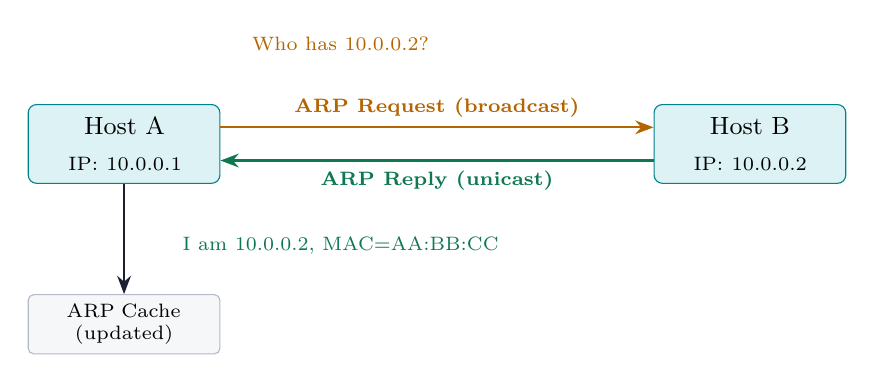
\begin{tikzpicture}[
  dev/.style={rectangle, draw=myteal, fill=hdrteal, text width=2.2cm, align=center, minimum height=1.0cm, font=\small, rounded corners=3pt},
  node distance=0.6cm
]
\node[dev] (A) {Host A\\[2pt]{\scriptsize IP: 10.0.0.1}};
\node[dev, right=5.5cm of A] (B) {Host B\\[2pt]{\scriptsize IP: 10.0.0.2}};

% ARP Request — above, with label above the arrow
\draw[-Stealth, thick, color=myamber]
  ([yshift=6pt]A.east) -- ([yshift=6pt]B.west)
  node[midway, above, font=\scriptsize\bfseries\color{myamber}] {ARP Request (broadcast)};
\node[font=\scriptsize\color{myamber}, above=0.55cm of A, xshift=2.75cm]
  {Who has 10.0.0.2?};

% ARP Reply — below, with label below the arrow
\draw[-Stealth, thick, color=mygreen]
  ([yshift=-6pt]B.west) -- ([yshift=-6pt]A.east)
  node[midway, below, font=\scriptsize\bfseries\color{mygreen}] {ARP Reply (unicast)};
\node[font=\scriptsize\color{mygreen}, below=0.55cm of A, xshift=2.75cm]
  {I am 10.0.0.2, MAC=AA:BB:CC};

% Cache
\node[rectangle, draw=mgframe, fill=mygray, text width=2.2cm, align=center,
  font=\scriptsize, below=1.4cm of A, rounded corners=2pt] (cache) {ARP Cache\\(updated)};
\draw[arrow] (A.south) -- (cache.north);
\end{tikzpicture}
\end{tcolorbox}

\textbf{IPv4 vs.\ IPv6 Key Differences:}\par\noindent
\begin{tabularx}{\linewidth}{|B{3.0cm}|X|X|}
\hline
\multicolumn{1}{|>{\centering\arraybackslash}p{3.0cm}|}{\textbf{Feature}} &
\multicolumn{1}{>{\centering\arraybackslash}X|}{\textbf{\color{myteal}IPv4}} &
\multicolumn{1}{>{\centering\arraybackslash}X|}{\textbf{\color{myamber}IPv6}} \\
\hline
Address size    & 32 bits (4 bytes)             & 128 bits (16 bytes) \\
\hline
Notation        & Dotted decimal (x.x.x.x)      & Colon-hex (x:x:x:x:x:x:x:x) \\
\hline
Header size     & 20--60 bytes (variable)        & 40 bytes (fixed) \\
\hline
Fragmentation   & By routers and hosts           & By source host only \\
\hline
Checksum        & Present in header              & Removed (handled by upper layers) \\
\hline
Security        & Optional (IPSec)               & Mandatory (IPSec built-in) \\
\hline
\end{tabularx}

%═══════════════════════════════════════════════════════════════════════════════
\section{Transport Layer}
%═══════════════════════════════════════════════════════════════════════════════

\begin{tcolorbox}[defbox]
\textbf{Transport Layer (Layer 4):} Provides \textit{process-to-process} (end-to-end) delivery of data. Handles segmentation, reassembly, flow control, error control, and multiplexing using \textbf{port numbers}.
\end{tcolorbox}

\subsection{UDP (User Datagram Protocol)}

\begin{tcolorbox}[formulabox, title={\textbf{UDP --- Connectionless, Unreliable}}]
\textbf{Features:} No connection setup, no acknowledgement, no flow/error control. Minimal overhead.\\
\textbf{Header:} 8 bytes --- Source Port (16b) $|$ Destination Port (16b) $|$ Length (16b) $|$ Checksum (16b).\\
\textbf{Use cases:} DNS, DHCP, SNMP, VoIP, video streaming, online gaming.\\
\textbf{Advantage:} Very fast, low latency. \textbf{Disadvantage:} No reliability guarantee.
\end{tcolorbox}

\subsection{TCP (Transmission Control Protocol)}

\begin{tcolorbox}[formulabox, title={\textbf{TCP --- Connection-Oriented, Reliable}}]
\textbf{Features:} Full-duplex, byte-stream, reliable delivery, flow control (sliding window), congestion control, ordered delivery.\\
\textbf{Header:} 20--60 bytes. Key fields: Source/Dest Port, Sequence No., ACK No., Flags (SYN, ACK, FIN, RST), Window Size, Checksum.\\
\textbf{Use cases:} HTTP, FTP, SMTP, SSH, Telnet.
\end{tcolorbox}

\textbf{TCP Three-Way Handshake (Connection Establishment):}
\begin{enumerate}[label=\textbf{\arabic*.}, leftmargin=*, itemsep=3pt]
  \item \textbf{SYN:} Client sends SYN segment with initial sequence number $x$.
  \item \textbf{SYN-ACK:} Server responds with SYN ($y$) + ACK ($x+1$).
  \item \textbf{ACK:} Client sends ACK ($y+1$). Connection established.
\end{enumerate}

\textbf{TCP Connection Termination (Four-Way):} FIN $\to$ ACK $\to$ FIN $\to$ ACK.

\begin{tcolorbox}[tikzbox, title={TCP Three-Way Handshake}]
\centering
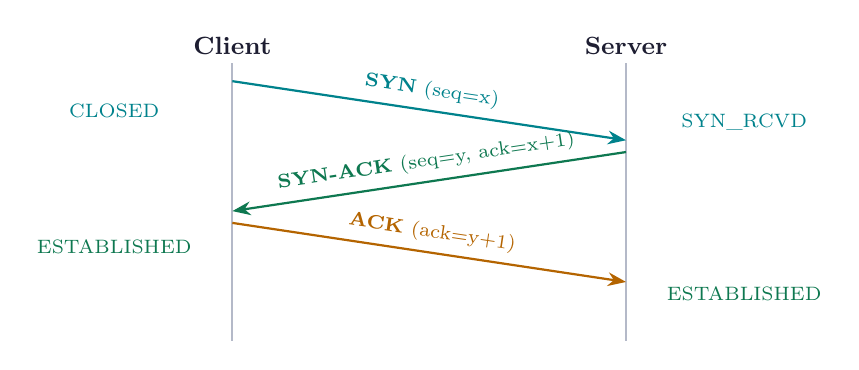
\begin{tikzpicture}[x=1cm, y=0.75cm,
  lbl/.style={font=\small\bfseries\color{mydark}},
  msg/.style={font=\scriptsize\color{mydark}}
]
\node[lbl] at (0,5.2) {Client};
\node[lbl] at (5,5.2) {Server};
\draw[thick,color=mgframe] (0,4.9) -- (0,0.2);
\draw[thick,color=mgframe] (5,4.9) -- (5,0.2);
% SYN
\draw[arrow,color=myteal] (0,4.6) -- node[above,sloped,msg]{\textbf{SYN} (seq=x)} (5,3.6);
\node[msg,color=myteal] at (-1.5,4.1) {CLOSED};
\node[msg,color=myteal] at (6.5,3.9) {SYN\_RCVD};
% SYN-ACK
\draw[arrow,color=mygreen] (5,3.4) -- node[above,sloped,msg]{\textbf{SYN-ACK} (seq=y, ack=x+1)} (0,2.4);
% ACK
\draw[arrow,color=myamber] (0,2.2) -- node[above,sloped,msg]{\textbf{ACK} (ack=y+1)} (5,1.2);
\node[msg,color=mygreen] at (-1.5,1.8) {ESTABLISHED};
\node[msg,color=mygreen] at (6.5,1.0) {ESTABLISHED};
\end{tikzpicture}
\end{tcolorbox}

\subsection{Congestion Control}

\begin{tcolorbox}[defbox]
\textbf{Congestion:} A state where the network cannot handle the offered load; routers drop packets, causing retransmissions and further congestion. Congestion control prevents/reduces this.
\end{tcolorbox}

\subsubsection*{Open Loop Congestion Control}
Prevents congestion \textbf{before it occurs} through good design policies:
\begin{itemize}[leftmargin=*, itemsep=3pt]
  \item \textbf{Retransmission policy:} Retransmit only when necessary (use timers wisely).
  \item \textbf{Window policy:} Use selective repeat (wastes less bandwidth than GBN).
  \item \textbf{Discarding policy:} Routers discard less sensitive packets first.
  \item \textbf{Acknowledgement policy:} Receiver delays ACK to reduce ACK traffic.
  \item \textbf{Admission policy:} Routers reject new connections if network is near capacity.
\end{itemize}

\subsubsection*{Closed Loop Congestion Control}
Reacts to congestion \textbf{after it occurs}:
\begin{itemize}[leftmargin=*, itemsep=3pt]
  \item \textbf{Backpressure:} Congested node sends a signal to upstream node to slow down. Works hop-by-hop.
  \item \textbf{Choke packet:} Congested router sends a choke packet directly to the source to reduce its transmission rate.
  \item \textbf{Implicit signalling:} Source detects congestion from dropped packets or increased delay (TCP's approach).
  \item \textbf{Explicit signalling:} Router sets a bit in the packet header to warn source/destination (ECN --- Explicit Congestion Notification).
\end{itemize}

\subsection{Quality of Service (QoS)}

\begin{tcolorbox}[defbox]
\textbf{QoS:} The ability of a network to provide different levels of service to different traffic types. Key metrics: \textbf{bandwidth}, \textbf{delay}, \textbf{jitter} (delay variation), \textbf{packet loss}.
\end{tcolorbox}

\subsubsection*{Leaky Bucket Algorithm}
\begin{tcolorbox}[formulabox, title={\textbf{Leaky Bucket Algorithm}}]
\textbf{Concept:} A bucket with a small hole at the bottom. Packets enter the bucket (queue) at any rate; they leave at a \textbf{constant rate} (the leak rate). Smooths bursty traffic into a steady stream.\\[4pt]
\textbf{Operation:}
\begin{itemize}[leftmargin=*, itemsep=2pt, topsep=0pt]
  \item If bucket is not full: incoming packet is added to the queue.
  \item If bucket is full: packet is \textbf{discarded} (overflow).
  \item Packets leave the bucket at a fixed rate $r$ (tokens/second).
\end{itemize}
\textbf{Advantage:} Enforces constant output rate. \textbf{Disadvantage:} Cannot handle bursts; excess packets dropped.
\end{tcolorbox}

\begin{tcolorbox}[tikzbox, title={Leaky Bucket vs Token Bucket}]
\centering
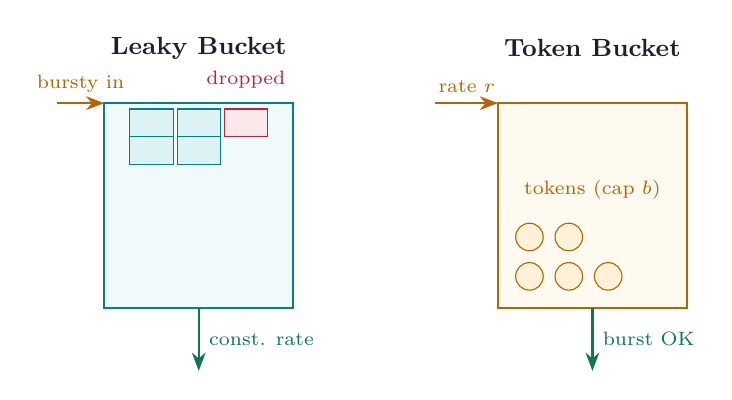
\begin{tikzpicture}[
  pkt/.style={rectangle, draw=myteal, fill=hdrteal, minimum width=0.55cm, minimum height=0.35cm, font=\tiny},
  tok/.style={circle, draw=myamber, fill=hdramber, minimum size=0.35cm, font=\tiny},
  lbl/.style={font=\small\bfseries\color{mydark}}
]
%--- Leaky Bucket (left) ---
\node[lbl] at (1.5,4.5) {Leaky Bucket};
% bucket outline
\draw[thick,color=myteal,fill=hdrteal!40] (0.3,1.2) -- (0.3,3.8) -- (2.7,3.8) -- (2.7,1.2) -- cycle;
% packets entering (bursty)
\foreach \y in {3.2,3.55} { \node[pkt] at (0.9,\y) {}; }
\foreach \y in {3.2,3.55} { \node[pkt] at (1.5,\y) {}; }
\node[pkt,draw=myred,fill=hdrred] at (2.1,3.55) {};
\node[font=\scriptsize\color{myred}] at (2.1,4.1) {dropped};
% arrows in
\draw[arrow,color=myamber] (-0.3,3.8) -- node[above]{\scriptsize bursty in} (0.3,3.8);
% hole at bottom
\draw[thick,color=myteal] (1.3,1.2) -- (1.7,1.2);
\draw[arrow,color=mygreen] (1.5,1.2) -- node[right]{\scriptsize const. rate} (1.5,0.4);

%--- Token Bucket (right) ---
\node[lbl] at (6.5,4.5) {Token Bucket};
\draw[thick,color=myamber,fill=hdramber!40] (5.3,1.2) -- (5.3,3.8) -- (7.7,3.8) -- (7.7,1.2) -- cycle;
% tokens
\foreach \x/\y in {5.7/1.6, 6.2/1.6, 6.7/1.6, 5.7/2.1, 6.2/2.1} { \node[tok] at (\x,\y) {}; }
\node[font=\scriptsize\color{myamber}] at (6.5,2.7) {tokens (cap $b$)};
% token generator
\draw[arrow,color=myamber] (4.5,3.8) -- node[above]{\scriptsize rate $r$} (5.3,3.8);
% packet consumes token
\draw[arrow,color=mygreen] (6.5,1.2) -- node[right]{\scriptsize burst OK} (6.5,0.4);
\end{tikzpicture}
\end{tcolorbox}

\subsubsection*{Token Bucket Algorithm}
\begin{tcolorbox}[formulabox, title={\textbf{Token Bucket Algorithm}}]
\textbf{Concept:} Tokens are generated at a constant rate $r$ and stored in a bucket (capacity $b$). A packet can only be sent if a token is available (one token consumed per packet).\\[4pt]
\textbf{Operation:}
\begin{itemize}[leftmargin=*, itemsep=2pt, topsep=0pt]
  \item Tokens accumulate up to bucket capacity $b$.
  \item To send a packet: remove one token from bucket.
  \item If no token available: packet must wait (or be discarded).
\end{itemize}
\textbf{Maximum burst size:} $b$ packets (when bucket is full).\\
\textbf{Advantage:} Allows controlled bursts up to $b$. More flexible than leaky bucket.
\end{tcolorbox}

\begin{tabularx}{\linewidth}{|B{3.0cm}|X|X|}
\hline
\multicolumn{1}{|>{\centering\arraybackslash}p{3.0cm}|}{\textbf{Feature}} &
\multicolumn{1}{>{\centering\arraybackslash}X|}{\textbf{\color{myteal}Leaky Bucket}} &
\multicolumn{1}{>{\centering\arraybackslash}X|}{\textbf{\color{myamber}Token Bucket}} \\
\hline
Output rate     & Constant (fixed)              & Variable (up to burst limit) \\
\hline
Burst handling  & Excess packets dropped        & Bursts allowed up to $b$ tokens \\
\hline
Flexibility     & Less flexible                 & More flexible \\
\hline
Use case        & Traffic shaping               & Traffic policing with burst allowance \\
\hline
\end{tabularx}

%═══════════════════════════════════════════════════════════════════════════════
% QUICK REVISION PAGE
%═══════════════════════════════════════════════════════════════════════════════
\newpage
\begin{center}
  {\large\bfseries\color{myred} Quick Revision --- Module 3}\\[3pt]
  {\small\color{mydark} Network Layer \& Transport Layer $|$ EC602}
\end{center}
\noindent{\color{myred}\rule{\linewidth}{1.2pt}}
\vspace{4pt}

\begin{tcolorbox}[formulabox, title={\textbf{Key Facts at a Glance}}]
\begin{tabularx}{\linewidth}{B{5.0cm} X}
Class A range           & 1--126; mask 255.0.0.0 \\[2pt]
Class B range           & 128--191; mask 255.255.0.0 \\[2pt]
Class C range           & 192--223; mask 255.255.255.0 \\[2pt]
Subnets                 & $2^s$ (s = borrowed bits) \\[2pt]
Hosts per subnet        & $2^h - 2$ (h = host bits) \\[2pt]
RIP metric / max hops   & Hop count / 15 \\[2pt]
OSPF metric             & Cost (bandwidth-based) \\[2pt]
BGP use                 & Inter-AS routing; TCP port 179 \\[2pt]
ARP function            & IP $\to$ MAC address resolution \\[2pt]
ICMP use                & Error reporting; ping (Echo Request/Reply) \\[2pt]
IPv6 address size       & 128 bits \\[2pt]
TCP handshake           & SYN $\to$ SYN-ACK $\to$ ACK \\[2pt]
UDP header size         & 8 bytes \\[2pt]
TCP header size         & 20--60 bytes \\[2pt]
Leaky bucket output     & Constant rate \\[2pt]
Token bucket burst      & Up to $b$ tokens \\[2pt]
\end{tabularx}
\end{tcolorbox}

\vspace{6pt}

\begin{tcolorbox}[defbox, title={\textbf{One-Line Definitions}}]
\begin{itemize}[leftmargin=*, itemsep=3pt, topsep=0pt]
  \item \textbf{Router:} Layer 3 device that routes packets between networks using IP addresses.
  \item \textbf{Gateway:} Protocol converter connecting networks with different protocols.
  \item \textbf{Subnetting:} Dividing a network into smaller subnets by borrowing host bits.
  \item \textbf{RIP:} Distance vector routing protocol; metric = hop count; max 15 hops.
  \item \textbf{OSPF:} Link state routing protocol; uses Dijkstra's algorithm; metric = cost.
  \item \textbf{BGP:} Path vector protocol for inter-AS routing on the Internet.
  \item \textbf{ARP:} Resolves IP address to MAC address via broadcast.
  \item \textbf{ICMP:} Reports network errors and provides diagnostic functions (ping).
  \item \textbf{TCP:} Reliable, connection-oriented transport protocol with flow/error control.
  \item \textbf{UDP:} Unreliable, connectionless transport protocol; low overhead, fast.
  \item \textbf{Congestion:} Network overload causing packet drops and retransmissions.
  \item \textbf{Leaky Bucket:} Traffic shaping algorithm enforcing constant output rate.
  \item \textbf{Token Bucket:} Traffic policing algorithm allowing controlled bursts.
\end{itemize}
\end{tcolorbox}

\vspace{6pt}

\begin{tcolorbox}[exambox, title={\textbf{Frequently Asked / Viva Questions}}]
\begin{enumerate}[leftmargin=*, topsep=0pt, label=\textbf{Q\arabic*.}, itemsep=8pt]
  \item \Q{What is the difference between a switch and a router?} Switch operates at Layer 2 (MAC addresses, within a network); router operates at Layer 3 (IP addresses, between networks).
  \item \Q{What is subnetting and why is it used?} Dividing a network into smaller subnets. Used to reduce broadcast domains, improve security, and efficient IP address utilisation.
  \item \Q{How many hosts can a /26 subnet support?} $2^6 - 2 = 62$ usable hosts.
  \item \Q{Difference between RIP and OSPF?} RIP: distance vector, hop count metric, max 15 hops, slow convergence. OSPF: link state, cost metric, no hop limit, fast convergence.
  \item \Q{What is BGP used for?} Inter-domain routing between Autonomous Systems on the Internet; uses path vector algorithm.
  \item \Q{What does ARP do?} Resolves an IP address to a MAC address by broadcasting an ARP request on the local network.
  \item \Q{Difference between TCP and UDP?} TCP: reliable, connection-oriented, ordered, flow/error control. UDP: unreliable, connectionless, no ordering, minimal overhead.
  \item \Q{What is the TCP three-way handshake?} SYN (client) $\to$ SYN-ACK (server) $\to$ ACK (client). Establishes a reliable connection.
  \item \Q{What is the difference between leaky bucket and token bucket?} Leaky bucket: constant output rate, excess dropped. Token bucket: variable output up to burst size $b$, more flexible.
  \item \Q{What is a choke packet?} A packet sent by a congested router directly to the source to reduce its transmission rate (closed-loop congestion control).
  \item \Q{What is the purpose of TTL in IP header?} Time To Live; decremented by each router. When TTL = 0, packet is discarded. Prevents infinite routing loops.
  \item \Q{What are the main improvements of IPv6 over IPv4?} 128-bit addressing, fixed 40-byte header, no router fragmentation, built-in IPSec, no broadcast (uses multicast).
\end{enumerate}
\end{tcolorbox}

\end{document}
